
\begin{lemma}{Mitternachtsformel}
    $x=\frac{-b\pm\sqrt{b^2-4ac}}{2a}$
\end{lemma}

\begin{theorem}{Polynomdivision} \emph{!} Vorzeichen von Nullstellen umdrehen\\
    $\frac{P(x)}{q(x)} = S(x) + \frac{r(x)}{q(x)}$ \qquad $P,q,S,r$ Polynome
\end{theorem}


\raggedcolumns
\subsubsection{Trigonometrische Funktionen}

\begin{iequation}[align*]
	\tikz[remember picture] \coordinate(sinanchor) at (0,0); \sin x &= \sum_{n=0}^{\infty} \frac{(-1)^n x^{2n + 1}}{(2n+1)!} = x - \frac{x^3}{3!} + \frac{x^5}{5!}\ldots ~ \text{stetig}\\
	\tikz[remember picture] \coordinate(cosanchor) at (0,0); \cos x &= \sum_{n=0}^{\infty} \frac{(-1)^n x^{2n}}{(2n)!} = 1 - \frac{x^2}{2!} + \frac{x^4}{4!}\ldots \hspace{3.8mm} \text{stetig}\\
	\tan x &= \frac{\sin x}{\cos x} \hspace{10mm} \cot x = \frac{\cos x}{\sin x} \tikz[remember picture] \coordinate(trigfunkanchor) at (0,0);
\end{iequation}
\begin{tikzpicture}[remember picture, overlay]
	\node[overlaynote, text width = 28mm, anchor = west] at ($(trigfunkanchor) + (0.5,0.25)$) {$\pi$: kleinste strikt positive Nullstelle von $\sin$.};
	\node[overlaynote, rotate = 90] at ($(trigfunkanchor) + (3,2)$) {$\cos(x) = \sin (x + \frac{\pi}{2})$};
	\node[overlaynote, rotate = 20, above left = 3mm and 2mm of sinanchor] (sinnote) {ungerade};
	\draw[overlayarrow] (sinnote) to[bend right] (sinanchor);
	\node[overlaynote, rotate = 20, above left = 3mm and 2mm of cosanchor] (cosnote) {gerade};
	\draw[overlayarrow] (cosnote) to[bend right] (cosanchor);
\end{tikzpicture}






\begin{theorem}{Eigenschaften sin/cos}
    \begin{itemize}
        \item $\cos x = \cos(-x) ~\text{und}~ \sin(-x) = -\sin x \quad\forall x \in \mathbb{C}$
        \item $\sin(x + y) = \sin(x)\cos(y) + \cos(x)\sin(y)$
        \item $\cos(x + y) = \cos(x)\cos(y) - \sin(x)\sin(y)$
        \item $\sin^2(x) = \frac{1 - \cos(2x)}{2} \quad \cos^2(x) = \frac{1 + \cos(2x)}{2}$
        \item $\cos^2(x) + \sin^2(x) = 1 \quad \forall x \in \mathbb{C}$ 
        \item $\sin(2x) = 2 \sin(x)\cos(x)$ \hspace{4mm} $\cos(2x) = \cos^2(x) - \sin^2(x)$
    \end{itemize} 
 \end{theorem}
 
 \begin{corollary}{Eigenschaften mit $\pi$}
     \begin{enumerate}[itemsep= 2pt]
         \item $\sin(x + \frac{\pi}{2}) = \cos(x), \quad \cos(x + \frac{\pi}{2}) = -\sin(x)$
         \item $\sin(x+\pi) = -\sin (x), \quad \sin(x + 2\pi) = \sin(x)$
         \item $\cos(x+\pi) = -\cos (x), \quad \cos(x + 2\pi) = \cos(x)$
     \end{enumerate}
 \end{corollary}

 \begin{corollary}{Nullstellen von trigonometrischen Funktionen}
    \begin{enumerate}
         \item $\text{Nullstellen Sinus} = \{k\cdot \pi : k\in \mathbb{Z}\}$\\
        $\sin(x) > 0 \quad \forall x \in ]2k\pi, ~(2k+1)\pi[, ~ k\in \mathbb{Z}$\\[2pt]
        $\sin(x) < 0 \quad \forall x \in ](2k + 1)\pi, ~(2k+2)\pi[, ~ k\in \mathbb{Z}$
        \item $\text{Nullstellen Cosinus} = \left\{\frac{\pi}{2}+k\cdot \pi : k\in \mathbb{Z}\right\}$\\
        $\cos(x) > 0:\forall x \in \left]-\frac{\pi}{2} +2k\pi, ~-\frac{\pi}{2} +(2k+1)\pi\right[, ~ k\in \mathbb{Z}$\\[2pt]
        $\cos(x) < 0:\forall x \in \left]-\frac{\pi}{2} + (2k + 1)\pi, ~-\frac{\pi}{2} +(2k+2)\pi\right[, ~ k\in \mathbb{Z}$
    \end{enumerate}
\end{corollary}
 


\subsubsection*{Logarithmen}
\begin{concept}{Rechnen mit Logarithmen}
    \begin{itemize}
        \item $\ln (a \cdot b) = \ln a + \ln b \quad \forall a,b \in ]0 +  \infty[$
        \item $\ln (a \div b) = \ln a - \ln b \quad \forall a,b \in ]0 +  \infty[$
        \item ${\ln (x^a) = a \ln (x) \quad \forall a \in \R, \forall x > 0}$
    \end{itemize}
    Im Allgemeinen gilt: $log_b (a) = \frac{ln(a)}{ln(b)}$
\end{concept}

\begin{formula}{ln(1 + x)}
       $ = \sum_{n=1}^\infty \frac{(-1)^{n-1}x^n}{n} \quad \text{für} \quad |x| < 1$
\end{formula}

\begin{KR}{Logarithmus abschätzen}\\
    $\log_b (n)$ kann mit $n^\alpha$ ($\alpha > 0$) abgeschätzt werden.\\
    $\ln(n) \leq \sqrt{n}$
\end{KR} 



\section{Funktionen und Konvergenz}

\raggedcolumns

\begin{definition}
    {Komposition/Verkettung} $(g \circ f)(x)=g(f(x))$
\end{definition}


\begin{definition}{Symmetrie} gerade $f(-x)=f(x)$, ungerade $f(-x)=-f(x)$
\end{definition}


\begin{definition}{Stetigkeit}
    Eine Funktion ist stetig, falls die Kurve keine Sprünge macht und man den Graphen der Funktion zeichnen kann, ohne den Stift dabei abzusetzen.
\end{definition}

\begin{definition}{Gleichmässige Konvergenz} für alle Werte der Funktion gilt:
    $$\lim_{x \to x_0^+} f(x) = \lim_{x \to x_0^-} f(x)$$
    (Linksseitiger Grenzwert = Rechtsseitiger Grenzwert)
\end{definition}


\begin{corollary}{Rechnen mit Grenzwerten von Funktionen}
    \begin{itemize}
        \item $\lim_{x \to x_0} (f + g)(x) = \lim_{x \to x_0} f(x) + \lim_{x \to x_0} g(x)$
        \item $\lim_{x \to x_0} (f \cdot g)(x) = \lim_{x \to x_0} f(x) \cdot \lim_{x \to x_0} g(x)$
        \item Sei $f \leq g$, so ist $\lim_{x \to x_0} f(x) \leq \lim_{x \to x_0} g(x)$
        \item Falls $g_1 \leq f \leq g_2$ und $\lim_{x \to x_0} g_1(x) = \lim_{x \to x_0} g_2(x)$, so existiert $\lim_{x \to x_0} f(x) = \lim_{x \to x_0} g_1(x)$
    \end{itemize}
\end{corollary}

\begin{definition}{Reihen - Funktionen}\\
        $
        \begin{array}{ll}
            \sum^{n}_{k=1} k = \frac{n \cdot (n+1)}{2} & \sum^{n}_{k=1} (2k - 1)^2 = \frac{n \cdot (4n^2-1)}{3}\\
            \sum^{n}_{k=1} 2k-1 = n^2 & \sum^{n}_{k=1} k^3 = ( \frac{n \cdot (n+1)}{2})^2\\
            \sum^{n}_{k=1} 2k = n(n+1) & \sum^{n}_{k=1} \frac{1}{k(k+1)} = \frac{n}{n+1}\\
            \sum^{n}_{k=1} k^2 = \frac{n \cdot (n+1) \cdot (2n+2)}{6} &
        \end{array}
        $
    \end{definition}



    \begin{formula}{Spezielle Grenzwerte}
        \textcolor{pink}{\[n\rightarrow \infty\]}
        \resizebox*{0.9\linewidth}{!}{
        %\def\arraystretch{1.2}
        \begin{tabular}{c|c|c}
            \(\frac{1}{n}\rightarrow 0\)& \(e^n\rightarrow \infty\)&\(\frac{1}{n^k}\rightarrow 0\ \ \forall k\in
            \mathbb{R}^+\)\\
            \hline
            \(c+\frac{1}{n}\rightarrow c\)&\(e^{-n}\rightarrow 0\)&\((1+n)^{\frac{1}{n}}\rightarrow 1\)\\
            \hline
            \(\frac{c\cdot n}{c^n}\rightarrow 0\)&\(\frac{e^n}{n^c}\rightarrow \infty\)&\((1+\frac{1}{n})^c
            \rightarrow 1\)\\
            \hline
        \(\sqrt[n]{n}=n^{\frac{1}{n}}\rightarrow 1\)&\(\frac{\sin{n}}{n}\rightarrow 0\)&\((1+\frac{1}{n})^n
        \rightarrow e\)\\
        \hline
        \(\sqrt[n]{n!}\rightarrow \infty\)&\(\arctan{n}\rightarrow \frac{\pi}{2}\)&\((1+\frac{c}{n})^n
        \rightarrow e^c\)\\
        \hline
        \(\frac{1}{n}\sqrt[n]{n!} \rightarrow \frac{1}{e}\)&\(\ln{n}\rightarrow \infty\)&\((1-\frac{1}{n} )^n
        \rightarrow \frac{1}{e}\)\\
        \hline
        \(\frac{c^n}{n!} \rightarrow 0\)&\(\frac{\ln{n}}{n}\rightarrow 0\)&\((\frac{n}{n+c})^n\rightarrow
        e^{-c}\)\\
        \hline
        \(\frac{n^n}{n!}\rightarrow \infty\)&\(\frac{\log{n}}{n-1}\rightarrow 1\)& \\
        \end{tabular}
        }
        \[n^c\cdot q^n \rightarrow 0 \quad \forall c \in \mathbb{Z},0\leq q \leq 1\]
        \[n(\sqrt[n]{c}-1)\rightarrow \ln{c}\quad \forall c > 0\]
        \textcolor{pink}{\[n\rightarrow 0\]}
        \resizebox*{0.9\linewidth}{!}{
        %\def\arraystretch{1.2}
        \begin{tabular}{c|c|c}
            \(\ln{n}\rightarrow -\infty\)&\(\frac{\sin{n}}{n}\rightarrow 1\)&\(\frac{1}{\arctan{n}}\rightarrow 1\)\\
            \hline
            \(n\log{n}\rightarrow 0\)&\(\frac{\cos{(n)}-1}{n}\rightarrow 0\)&\(\frac{e^n-1}{n}\rightarrow 1\)\\
            \hline
            \(\frac{\log{1}-n}{n}\rightarrow -1\)&\(\frac{1}{\cos{n}}\rightarrow1\)&\(\frac{e^cn-1}{n}\rightarrow c\)\\
            \hline 
            \(\frac{c^n-1}{n}\rightarrow\ln{c},\forall c>0\)&\(\frac{1-\cos{n}}{n^2}\rightarrow
            \frac{1}{2}\)&\((1+n)^{\frac{1}{n}}\rightarrow e\)\\
        \end{tabular}
        }
    \end{formula}

\raggedcolumns


\section{Taylorrreihen}

\begin{definition}{Potenzreihe} undendliche Reihe vom Typ:
    \begin{center}
    $p(x)=a_0+a_1x+a_2x^2+ \cdots = \sum_{k=0}^{\infty}{a_kx^k} $\\
    \vspace{2mm}
    \(a_0,a_1, \cdots \in \R\) sind die Koeffizienten der Potenzreihe
    \end{center}
    Allgemein kann eine Potenzreihe mit einer Verschiebung von \(x_0\) beschrieben werden $\Rightarrow$ Potenzreihe mit Zentrum \(x_0\):
    \begin{center}
    $p(x)=a_0+a_1(x-x_0)+a_2(x-x_0)^2+\cdots = \sum_{k=0}^{\infty}{a_k(x-x_0)^k}$
    \end{center}
\end{definition}

\begin{definition}{Taylorreihe} oder Taylorentwicklung einer Funktion \(y=f(x)\) and der Stelle \(x_0\) ist die Potenzreihe:
  \begin{center}
    $t_f(x)=\sum_{k=0}^{\infty}{a_k(x-x_0)^k}$
  \end{center}
  welche die gleiche Ableitung an der Stelle \(x_0 \text{ für alle }k\in \mathbb{N}\) hat wie die Funktion \(f(x)\)
\end{definition}

\begin{definition}{Taylorpolynom}
  ist eine Taylorreihe \(t_f(x)\) welche nach \(n\text{-ter}\) Ordnung abgebrochen wird.
        Somit erhällt man das Taylorpolynom \(n\text{-ter}\) Ordnung von \(f(x)\) an der Stelle \(x_0\):
    \begin{center}
    $p_n(x)=\sum_{k=0}^{n}{a_k(x-x_0)^k}$
    \end{center}
    Bemerkung: Die Tangente der Funktionskurve \(y=f(x) \) an der Stelle \(x_0\) ist exakt das Taylorpolynom 1.
      Ordnung von \(f(x)\) an der Stelle \(x_0\)
\end{definition}

\begin{KR}{Vorgehen Berechnen Taylorreihe}
  Die Taylorreihe einer beliebig oft differenzierbaren Funktion \(t(x)\) an der Stelle \(x_0\) ist:
  \[t_f(x) = \sum_{k=0}^{\infty}{\frac{f^{k}(x_0)}{k!}\cdot(x-x_0)^k}\]
\end{KR}

\begin{formula}{Formel für Taylorkoeffizienten} 
  Formel für \(k\)-ten Taylorkoeffizientn der Taylorreihe \(t_f(x)\) von \(f(x)\) an der Stelle
  \(x_0\in\mathbb{R}\):
  \[a_k=\frac{f^{(k)}(x_0)}{k!}\quad (k\in\mathbb{N})\]
\end{formula}

\begin{theorem}{Taylorreihen wichtiger Funktionen}\\
    \def\arraystretch{2}
  \begin{tabular}{c}
  \(f(x)=e^x \text{ mit }x_0=0,\)\\\(t_f(x)=\sum_{k=0}^{\infty}{\frac{x^k}{k!}}=1+x+\frac{x^2}{2!}+\frac{x^3}{3!}\ldots\)\\
  \hline
  \(f(x)=\sin{(x)}\text{ mit }x_0=0,\)\\\(  t_f(x)=\sum_{k=0}^{\infty}{(-1)^k\frac{x^{2k+1}}{(2k+1)!}}=x-\frac{x^3}{3!}+\frac{x^5}{5!}-\ldots\)\\
  \hline
  \(f(x)=\cos{(x)}\text{ mit }x_0=0,\)\\\(
  t_f(x)=\sum_{k=0}^{\infty}{(-1)^k\frac{x^{2k}}{(2k)!}}=1-\frac{x^2}{2!}+\frac{x^4}{4!}-\ldots\)\\
  \hline
  \(f(x)=\ln{(x)}\text{ mit }x_0=1,\)\\\(
  t_f(x)=\sum_{k=1}^{\infty}{\frac{(-1)^{k+1}}{k}(x-1)^k}=(x-1)-\frac{(x-1)^2}{2}+\frac{(x-1)^3}{3}-\ldots\)\\
\end{tabular}
\end{theorem}


\subsubsection{Konvergenz von Potenzreihen}
\begin{definition}{Konvergenzradius}
  \begin{itemize}
    \item Der Konvergenzradius \(\rho\) einer Potenzreih\\ \(p(x)=\sum_{k=0}^{\infty}{a_k(x-x_0)^k}\) ist
      eine Zahl mit Folgenden Eigenschaften:
      \subitem - Für alle \(x\in\mathbb{R}\) mit \(|x-x_0|<\rho\) konvergiert die Reihe \(p(x)\)
      \subitem - Für alle \(x\in\mathbb{R}\) mit \(|x-x_0|>\rho\) divergiert die Reihe \(p(x)\)
    \item Es existieren folgende Extremfälle:
      \subitem - Konvergenzradius \(\rho = 0\): Dann konvergiert die Reihe \(p(x)\) nur für \(x=x_0\).
      \subitem - Konvergenzradius \(\rho = \infty\): Dann konvergiert die Reihe \(p(x)\) für alle \(x\in\mathbb{R}\).
  \end{itemize}
\end{definition}
\begin{formula}{Konvergenzradius Formel}\\
  Für die Potenzreihe \(\displaystyle p(x)=\sum_{k=0}^{\infty}{a_k(x-x_0)^k} \) ist der Konvergenzradius:
  \[\rho = \underset{k \rightarrow \infty}{\lim}\left| \frac{a_k}{a_{k+1}}\right| \quad \text{oder} \quad
  \rho=\underset{k \rightarrow \infty}{\lim} \frac{1}{\sqrt[k]{|a_k|} }\]
\end{formula}
\begin{formula}{Konvergenzbereich Formel}\\
  Der Konvergenzbereich in dem die Approximation der Funktion gilt ist definiert durch:
  \[(x_0 - \rho , x_0 + \rho) \]
\end{formula}


\section{Integralrechnung}

\begin{concept}{Integralregeln}
    \begin{itemize}
      \item Addition/Subtraktion:
      $\int f(x-k) d x=F(x-k)+C$
      \item Multiplikation:
      $\int f(x \cdot k) d x=\frac{1}{k} F(x \cdot k)+C$
      \item Skalarmultiplikation:
      $\int \lambda_{1} f(x)+\lambda_{2} g(x) d x=\lambda_{1} F(x)+\lambda_{2} G(x)+C$
      \item Linearkombination: \[\int{(\lambda_1f(x)+\lambda_2g(x))} = \lambda_2F(x)+\lambda_2G(x)+C \quad (\lambda_1,\lambda_2 \in \mathbb{R} )\]
      \item Verschiebung um k in x-Richtung: \[\int{f(x-k)\mathrm{d}x}= F(x-k)+C \quad (k \in \mathbb{R}) \]
      \item Streckung um k in x-Richtung: \[\int{f(k\cdot x)\mathrm{d}x}= \frac{1}{k}F(k\cdot x)+C \quad (k\neq0 )\]
    \end{itemize}
\end{concept}



\subsubsection{Integrationsmethoden}
\paragraph{Partielle Integration}

\begin{concept}{Partielle Integration}
	Seien $a < b$ reelle Zahlen und $f,g:[a,b] \to \R$ stetig differenzierbar. Dann gilt:
   \begin{equation*}
	   \int_a^b f(x) g'(x) \dif x = f(b) g(b) - f(a) g(a) - \int_a^b f'(x)g(x) \dif x
   \end{equation*}
   bzw. für unbestimmte Integrale\\

   $
   \int(f(x) \cdot g^{\prime}(x)) d x=f(x) \cdot g(x)-\int(f^{\prime}(x) \cdot g(x)) d x
   $
\end{concept}
\begin{remark}
   $\uparrow 1$ falls arc- oder log-Funktion vorkommt, $x^{n}, \frac{1}{1-x^{2}}, \frac{1}{1+x^{2}}$\\

   $\downarrow x^{n}, \arcsin (x), \arccos (x), \arctan (x)$,
\end{remark}
\begin{KR}{Prioritäten}$f(x)$ nach folgender Priorität auswählen:\\
   $
   \begin{array}{lllll}
	   1. \log_e, \log_a  & 2. \arcsin, \arccos &  3. x^2, 5x^3 & 4. \sin, \cos, \tan & 5. e^x, 5a^x
   \end{array}
   $
\end{KR}

\paragraph*{Substitution}

\begin{concept}{Substitution}\\
    Die Substitution ist die Umkehrung der Kettenregel. D.h. wir wollen Substitution vorallem verwenden, wenn wir innere Funktionen haben.
    \begin{equation*}
        \int_{g(b)}^{g(a)} f(x) \dif x = \int_{a}^b f(g(t)) g'(t) \dif t
    \end{equation*}
    bzw. für unbestimmte Integrale

    $$
    \int f(g(t)) \cdot g^{\prime}(t) d t=\left.\int f(x) d x\right|_{x=g(t)}
    $$
\end{concept}




\begin{corollary}{Nützliche Regeln}
	Sei $I \subseteq \R$ ein Intervall und $f: I \to \R$ stetig.
	\begin{enumerate}
		\item Seien $a,b,c \in \R$, sodass das abgeschlossene Intervall mit den Endpunkten $a+c$, $b+c$ in $I$ enthalten ist.
			Dann gilt
			\begin{equation*}
				\int_{a+c}^{b+c} f(x) \dif x = \int_{a}^{b} f(t+c) \dif t
			\end{equation*}
		\item Seien $a,b,c \in \R$ mit $c \neq 0$, sodass das abgeschlossene Intervall mit Endpunkten $ac$, $bc$ in $I$ enthalten ist.
			Dann gilt
			\begin{equation*}
				\int_{a}^{b} f(ct) \dif t = \frac{1}{c} \int_{ac}^{bc} f(x) \dif x
			\end{equation*}
	\end{enumerate}
\end{corollary}

\begin{KR}{Nützliche Substitutionen}
    \begin{itemize}
        \item $\log (x)$ subst: $t=\log (x), x=e^{t}, d x=e^{t} d t$
        \item für gerade $n: \cos ^{n}(x), \sin ^{n}(x), \tan (x)$ \\Sub: $t=\tan (x)$, $d y=\frac{1}{1+t^{2}} d t, \sin ^{2}(x)=\frac{t^{2}}{1+t^{2}}, \cos ^{2}(x)=\frac{1}{1+t^{2}}$
        \item für ungerade $n: \cos ^{n}(x), \sin ^{n}(x)$, \\Sub: $t=\tan (x / 2)$, $d y=\frac{2}{1+t^{2}} d t, \sin (x)=\frac{2 t}{1+t^{2}}, \cos (x)=\frac{1-t^{2}}{1+t^{2}}$
        \item $\int \sqrt{1-x^{2}} d x$ sub: $x=\sin (x)$ oder $\cos (x)$
        \item $\int \sqrt{1+x^{2}} d x$ sub: $x=\sinh (x)$
    \end{itemize}
\end{KR}




\begin{formula}{Substitution unbestimmtes Integral}
    \begin{itemize}
	\item Aufstellen und Ableiten der Substitutionsgleichungen:\\
	    $u=g(x),\quad \frac{\mathrm{d}u}{\mathrm{d}x}=g'(x),\quad \mathrm{d}x = \frac{\mathrm{d}u}{g'(x)} $
	\item Durchführen der Substitution \(u=g(x) \)	 und \(\mathrm{d}x=\frac{\mathrm{d}u}{g'(x)} \) in \\das  
	    integral $\int{f(x)\mathrm{d}x}$:
	    \[\int{f(x)\mathrm{d}x}=\int{r(u)}{\mathrm{d}u} \]
	\item Berechnen des Integrals mit Variable u:
	    $$\int{r(u)\mathrm{d}u}=R(u)+C$$
	\item Rücksubstitution:
	    $R(u)+C=R(g(x))+C$
    \end{itemize}	
\end{formula}

\begin{formula}{Substitution bestimmtes Integral}
    \begin{itemize}
	\item Aufstellen und Ableiten der Substitutionsgleichungen:\\
	    $u=g(x),\quad \frac{\mathrm{d}u}{\mathrm{d}x}=g'(x),\quad \mathrm{d}x = \frac{\mathrm{d}u}{g'(x)} $
	\item Durchführen der Substitution \(u=g(x) \)	 und \(\mathrm{d}x=\frac{\mathrm{d}u}{g'(x)} \) in \\das  
	    integral $\int{f(x)\mathrm{d}x}$:
	    \[\int_a^b{f(x)\mathrm{d}x}=\int_{g(a)}^{g(b)}{r(u)}{\mathrm{d}u} \]
	\item Berechnen des Integrals mit Variable u:
	    \[\int_{g(a)}^{g(b)}{r(u)\mathrm{d}u}=R(u)+C\Big|_{g(a)}^{g(b)} \]
	\item Rücksubstitution:
	    $$R(u)+C\Big|_{g(a)}^{g(b)}=R(g(x))+C\Big|_{g(a)}^{g(b)}$$
    \end{itemize}	
\end{formula}









\subsubsection*{Spezifische Aufgabenstellungen}

\begin{KR}{Integrieren von Flächen}
    Nullstellen bestimmen: $=>$ Fläche oberhalb $\mathrm{x}$ Achse, + Fläche evtl unterhalb x Achse...
    \end{KR}

\begin{KR}{Flächeninhalt bei wechselndem Vorzeichen von $f(x)$}\\
	\begin{itemize}
	  \item $[a, b]=$ Intervall
	  \item $x_{1}, x_{2}, \ldots, x_{n}=$ Nullstellen
	\end{itemize}
	
	$$\left|\int_{a}^{x_{1}} f(x) d x\right|+\left|\int_{x_{1}}^{x_{2}} f(x) d x\right|+\cdots+\left|\int_{x_{n}}^{b} f(x) d x\right|$$
	\end{KR}

	\begin{KR}{Flächeninhalt zwischen zwei Kurven $f(x)$ und $g(x)$}\\
		\begin{itemize}
		  \item $[a, b]=$ Intervall
		  \item $x_{1}, x_{2}, \ldots, x_{n}=$ Schnittpunkte
		\end{itemize}
		$$\left|\int_{a}^{x_{1}}(f(x)-g(x)) d x\right|+\left|\int_{x_{1}}^{x_{2}}(f(x)-g(x))\right|+\cdots+\left|\int_{x_{n}}^{b}(f(x)-g(x))\right|$$
		\end{KR}


\begin{theorem}{Mittelwert einer Funktion}\\
    \begin{center} %TODO make better graphic
    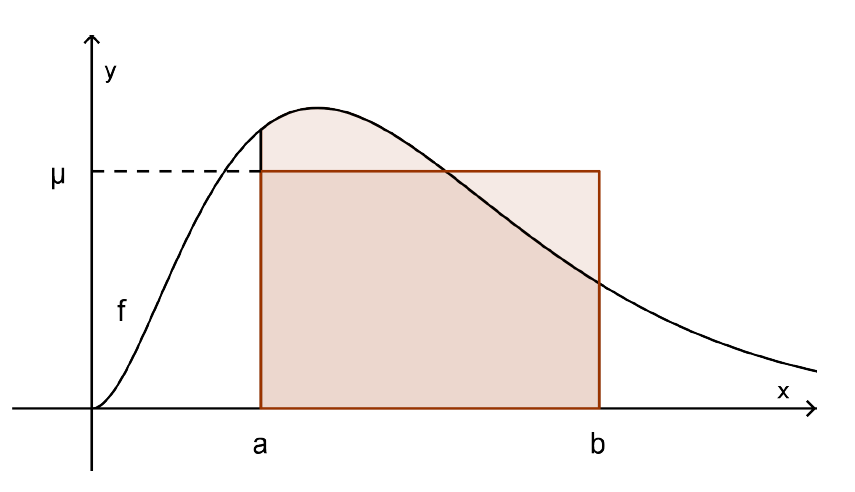
\includegraphics[width=0.4\linewidth]{Mittelwert_Grafik.png}
    \end{center}
  Definition des Mittelwert \(\mu\) der Funktion \(f(x)\) auf \([a,b]\): Höhe des Rechtecks, das
  \itemize
    \item eine Grundlinie der Länge \(b-a\) hat
    \item der Flächeninhalt des Rechteks der Fläche unter der Kurve \(f(x)\) im Intervall \([a,b]\) entspricht
	\[\mu = \frac{1}{b-a}\int_a^b{f(x)\mathrm{d}x} \]
\end{theorem}


\begin{theorem}{Schwerpunkt ebener Fläche}\\
  \begin{center}
  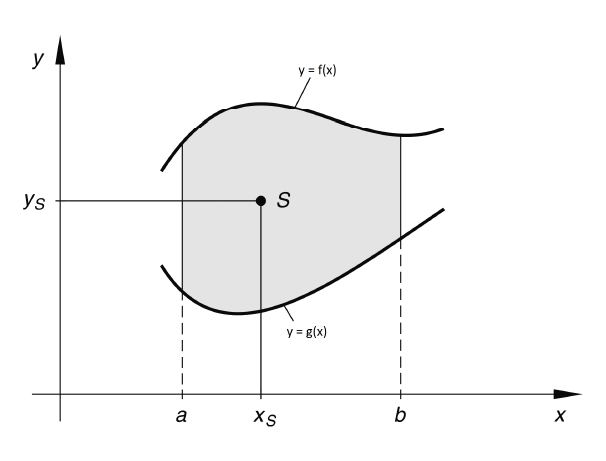
\includegraphics[width=0.4\linewidth]{Schwerpunkt_Beispiel.png}
  \end{center}
Schwerpunkt \(S=(x_s;y_s)\) einer ebenen Fläche mit Flächeninhalt A, eingegrenzt von Kurven \(y=f(x)\) und \(y=g(x)\)
sowie den Geraden \(x=a\) und \(x=b\):
\[xs = \frac{1}{A}\int_a^b{x\cdot(f(x)-g(x))\mathrm{d}x} \]
\[ys = \frac{1}{2A}\int_a^b{x\cdot(f(x)^2-g(x)^2)\mathrm{d}x} \]
Berechnen von \(A\) ebenfalls durch ein Integral:
\[A=\int_a^b{f(x)-g(x)\mathrm{d}x} \]
\end{theorem}
\begin{theorem}{Schwerpunkt Rotationskörper}\\
    Die x-Koordinate des Schwerpunkts \(S=(x_s;0;0) \) eines Rotationskörpers mit Volumen \(V\), geformt durch Rotation
    von \(y=f(x)\) zwischen \([a,b]\) um x-Achse mit \(a<b\) und \(f(x) \ge 0 \) für alle \(a \le x \le b \):
    \[x_s = \frac{\pi}{V}\int_a^b{x\cdot f(x)^2\mathrm{d}x} \]
\end{theorem}

\begin{formula}{Rotationsvolumen}
    $V = \pi \int_a^b{(f(x))^2\mathrm{d}x} $
\end{formula}
\begin{formula}{Bogenlänge}
    $L=\int_a^b{\sqrt{1+(f'(x))^2}\mathrm{d}x} $
\end{formula}
\begin{formula}{Mantelfläche}
    $M=2\pi \int_a^b{f(x)\cdot \sqrt{1+(f'(x))^2}\mathrm{d}x}$
\end{formula}

\raggedcolumns


\subsection{Uneigentliche Integrale}

\subsubsection{Uneigentliche Integrale erster Art}

\begin{KR}{Berechnung}
\begin{itemize}
	\item Rechnen mit endlichem Intervall \([a,\lambda] \text{ mit } \lambda \ge a \) anstelle von unendlichem
		Integral \([a,\infty) \)
		\[I(\lambda)=\int_a^{\lambda}{f(x)\mathrm{d}x} \]
	\item Das unendliche Intervall \([a,\infty) \) ergit sich aus \(\lim_{\lambda \rightarrow
		\infty}I(\lambda) \):
		\[I=\int_a^{\infty}{f(x)\mathrm{d}x}=\underset{\lambda \rightarrow \infty}{\lim}I(\lambda)=
		\underset{\lambda \rightarrow \infty}{\lim}(\int_a^{\lambda}{f(x)\mathrm{d}x}) \]
    \item Falls Grenzwert \(\underset{\lambda \rightarrow -\infty}{\lim}\) existiert, heisst das uneigentliche
        Integral \(\displaystyle\int_{a}^\infty {f(x)\mathrm{d}x}\) \(\bold{konvergent}\), andernfalls 
        \(\bold{divergent}\)
\end{itemize}
\end{KR}


\begin{KR}{Beidseitig unendliche Integrale}
\begin{itemize}
	\item Uneigentliche Integrale mit beidseitig unendlichen Integrationsinvervall:
		\[I=\int_{-\infty}^{\infty}{f(x)\mathrm{d}x}\]
	\item Einfügen einer künslichen Zwischengrenze \(c \in \mathbb{R}\\\text{typischerweise}\:c=0 \)
		\[\int_{-\infty}^{\infty}{f(x)\mathrm{d}x}=\int_{-\infty}^{c}{f(x)\mathrm{d}x}+\int_c^{\infty}
		{f(x)\mathrm{d}x} \]
	\item Beide Teilintegrale wie oben berechnen
	\item Das integral heisst \(\bold{konvergent}\) falls beide Teilintegrale konvergent sind.
\end{itemize}
\end{KR}

\subsubsection{Uneigentliche Integrale zweiter Art}
	\begin{definition}{Definition}\\
		Uneigentlich Integrale auf Interval \([a,b]\) mit einem Pol von \(f(x)\) bei \(x=a\) heisst,
		\(f(a) \rightarrow \infty\), und Stetigkeit auf \((a,b]\)
  \end{definition}
  \begin{KR}{Berechnung}
	  \begin{itemize}
	  	
\item Statt über \([a,b]\) integrieren, integrieren über \(a+\epsilon,b\) für beliebige \(\epsilon>0\):
	\[I(\epsilon)=\int_{a+\epsilon}^b{f(x)\mathrm{d}x}\]
\item Das Integral über \([a,b]\) ergibt sich aus \(\lim_{\epsilon \rightarrow 0}I(\epsilon)\):
	\[I=\int_a^b{f(x)\mathrm{d}x}=\underset{\epsilon \rightarrow 0}{\lim}I(\epsilon)=\underset{\epsilon \rightarrow
	0}{\lim}(\int_{a+\epsilon}^b{f(x)\mathrm{d}x}) \]
\item Das Integral heisst \(\bold{konvergent}\), falls der Limes \(\lim_{\epsilon \rightarrow 0}I(\epsilon)\) existiert.
\item Diese spezielle Variante ist nötig, weil beim Integralrechnen der Integral auf dem ganzen Intervall stetig sein
	muss. Dies ist nicht der Fall wen ein Pol existiert.
\end{itemize}
  \end{KR}


  \begin{formula}{Integraltabelle}\\
    \resizebox*{1.02\linewidth}{!}{
	\def\arraystretch{1.7}
	\begin{tabular}{c|c|c}
	    Ableitung | f'(x)                          & Funktion | f(x)                          & Integral | F(x)                       \\
        \hline
	    \(0\)                                      & \(C\)                                    & \(x+C\)                               \\
        \hline
        \(1\)                                      & \(x\)                                    & \(\frac{1}{2}x^2+C\)                  \\
        \hline
        \(-\frac{1}{x^2}\)                         & \(\frac{1}{x}\)                          & \(\ln|x|+C\)                          \\
        \hline
        \(ax^{a-1}\)                               & \(x^a \: with \: a \: \in \: \mathbb{R}\) & \(\frac{x^{a+1}}{a+1}+C\)             \\
        \hline
        $x^{x} \cdot(1+\ln x) \quad x>0$          & $x^{x}$                                  &   \\
        \hline
        $(x^{x})^{x}(x+2 x \ln (x)) \quad x>0$ & $x^{(x^{x})}$         &  \\
        \hline  
        
        $\frac{1}{2\sqrt{x}}$                     & $\sqrt{x}$                               &  $\frac{2}{3}x^{\frac{3}{2}}$         \\
        \hline
        $\frac{1}{n} x^{\frac{1}{n}-1}$           & $\sqrt[n]{x}$                            & $\frac{n}{n+1} x^{\frac{1}{n}+1}$     \\
        \hline

        \(\ln(a)\cdot a^x\)                       & \(a^x\)                                  & \(\frac{a^x}{\ln(a)}+C\)              \\
        \hline
        $a^{b x} \cdot c \ln a$                   & $a^{b x}$                                & $\frac{1}{b \ln a} a^{b x}$             \\
        \hline
        \(e^x\)                                   & \(e^x\)                                  & \(e^x+C\)                             \\
        \hline
        \(\frac{1}{x}\)                           & \(\ln(x)\)                               & \(x\ln(x)-x+C\)                       \\
        \hline
        \(\frac{1}{x\ln(a)}\)                     & \(\log_a(x)\)                            & \(x\log_a(x)-\frac{x}{\ln(a)}+C\)     \\
        \hline
        \(\cos(x)\)                                & \(\sin(x)\)                              & \(-\cos(x)+C\)                        \\
        \hline
        \(-\sin(x)\)                               & \(\cos(x)\)                              & \(\sin(x)+C\)                         \\
        \hline
        \(1+\tan^2{(x)=\frac{1}{\cos^2{(x)}}}\)    & \(\tan(x)\)                              & \(-\ln|\cos(x)|+C\)                   \\
        \hline
        \(-1-\cot^2{(x)}=-\frac{1}{\sin^2{(x)}}\)  & \(\cot(x)\)                              & \(\ln(\sin(x))+C\)                    \\
        \hline
        \(\frac{1}{\sqrt{1-x^2}}\)                & \(\arcsin(x)\)                           & \(x\arcsin(x)+\sqrt{1-x^2}+C\)        \\
        \hline
        \(-\frac{1}{\sqrt{1-x^2}}\)               & \(\arccos(x)\)                           & \(x\arccos(x)-\sqrt{1-x^2}+C\)        \\
        \hline
        \(\frac{1}{1+x^2}\)                       & \(\arctan(x)\)                           & \(x\arctan(x)-\frac{1}{2}\ln(1+x^2)+C\)\\
        %add more here
        \hline
        $\sin ^{2}(x)$                            & $\frac{1}{2}(x-\sin (x) \cos (x))$       & $\sin (x) \cos (x) + C$                   \\
        \hline
        $\cos ^{2}(x)$                            & $\frac{1}{2}(x+\sin (x) \cos (x))$       & $\cos (x) \sin (x) + C$                   \\ 
        \hline
        $\tan ^{2}(x)$                            & $\tan (x)-x$                             & $\tan (x) + C$                            \\
        \hline
        $\cot ^{2}(x)$                            & $-\cot (x)-x$                            & $\cot (x) + C$                            \\
        \hline
        $\frac{f'(x)}{f(x)}$                      & $\ln |f(x)|$                             & $x \cdot(\ln |x|-1) + C$                 \\
        \hline
        $\frac{1}{x}(\ln x)^{n}$                  & $\frac{1}{n+1}(\ln x)^{n+1} \quad n \neq-1$ & $\frac{1}{2 n}(\ln x^{n})^{2} \quad n \neq 0 + C$ \\
        \hline
        $\frac{1}{x \ln x}$                       & $\ln |\ln x| \quad x>0, x \neq 1$        & $\frac{1}{b \ln a} a^{b x} + C$           \\
        \hline
        $x \cdot e^{c x}$                         & $\frac{c x-1}{c^{2}} \cdot e^{c x}$      & $\frac{x^{n+1}}{n+1}(\ln x-\frac{1}{n+1}) \quad n \neq-1 + C$ \\
        \hline
        $x^{n} \ln x$                             & $\ln (\cosh (x))$                        & $\ln |f(x)| + C$                          \\
        \hline
        $\sin (x) \cos (x)$                       & $\frac{\sin^2(x)}{2} $                &\\
        \hline
        $\frac{-f^{\prime}(x)}{(f(x))^{2}}$       & $\frac{1}{f(x)}$                         & \\
        \hline
        $(a x+b)^{n}$                             & $\frac{1}{a \cdot(n+1)}(a x+b)^{n+1}$   & \\
        \hline
	\end{tabular}
    }
\end{formula}

\begin{KR}{Trick Gerade/Ungerade bei Integralen}\\
    Für ungerade Funktionen gilt $\int_{-a}^{+a} f(x) \dif x = 0$.
    \begin{itemize}
        \item Summe/Komposition: ungerade und ungerade $\rightarrow$ ungerade
        \item Produkt/Quotient: ungerade und gerade $\rightarrow$ ungerade
        \item Ableitung: gerade $\longrightarrow$ ungerade
    \end{itemize}
    Bsp ungerade: $f(x)$ = $-x$, $x$, $sin(x)$, $tan(x)$, Polynomfunktionen mit ungeradem Exponent\\
    gerade: $1$, $x^2$, $cos(x)$, $sec(x)$, Polynomf. mit geradem Exponent\\
    gerade und ungerade!! $f(x) = 0$
\end{KR}

\section{Differentialrechnung}




   

\subsubsection{Differentialquotient und Ableitung}


\begin{definition}{Sekanten-Steigung und Differentialquotient}
    $$\frac{\Delta f}{\Delta \mathrm{x}}=\frac{f(x_{0}+h)-f(x_{0})}{h}$$
\end{definition}

\begin{formula}{Tangentengleichung}
    $
    y=f^{\prime}(x_{0}) \cdot(x-x_{0})+f(x_{0})
    $
\end{formula}

\begin{definition}{Differenzierbarkeit}
    $f$ ist in $x_0$ \emph{differenzierbar}, falls der Grenzwert $\lim_{x \to x_0} \frac{f(x) -f(x_0)}{x -x_0}$ für alle 
    existiert.\\
    Den Grenzwert selbst bezeichnet man als Ableitung $f'(x)$ 
    \tcblower 
    \small
    Vereinfacht: Eine Funktion ist differenzierbar, falls die Kurve keine Knicke macht.
\end{definition}



\begin{definition}{Stetige Differenzierbarkeit}
	Eine Funktion ist stetig differenzierbar, wenn sie differenzierbar ist und ihre Ableitungsfunktion stetig ist.
\end{definition}


\begin{definition}{n-fache Differenzierbarkeit}
	\begin{enumerate}
		\item Für $n \geq 2$ ist $f$ \emph{$n$-mal differenzierbar} in $D$ falls $f^{n-1}$ in $D$ differenzierbar ist. Dann ist $f^{(n)} \coloneqq (f^{(n-1)})'$ 
		\item Die Funktion $f$ ist \emph{$n$-mal stetig differenzierbar} in $D$, falls sie $n$-mal differenzierbar ist und falls $f^{(n)}$ in $D$ stetig ist.
		\item Die Funktion $f$ ist in $D$ \emph{glatt}, falls sie $\forall n \geq 1$, $n$-mal differenzierbar ist. 
	\end{enumerate}
\end{definition}


\begin{itemize}
	\item $\exp$, $\sin$, $\cos$, $\sinh$, $\cosh$, $\tanh$ sind glatt auf $\R$
	\item Alle Polynome sind auf ganz $\R$ glatt
	\item $\ln : ]0, + \infty[ \to \R$ ist glatt
\end{itemize}


\begin{concept}{Ableitungsregeln}
    Seien $f,g: D \to \R$  differenzierbar. Dann gelten:
    \begin{itemize}
        \item Summe/Differenz: $(f + g)'(x) = f'(x) + g'(x)$
        \item Faktor: $f(x)=a\cdot g(x) \rightarrow f'(x)=a \cdot g'(x) $
        \item Produkt: $(f \cdot g)'(x) = f'(x)g(x) + f(x)g'(x)$
        \item Quotient: $(\frac{f}{g})'(x) = \frac{f'(x) g(x) - f(x) g'(x)}{g(x)^2}$
        \item Kettenregel: $(g \circ f)' (x) = g'(f(x)) f'(x)$
        \item Umkehrfunktion: $(f^{-1})'(y_0) = \frac{1}{f'(x)}$
        \item Potenz/Logarithmus 1: 
        $(a^{f(x)})' = ln(a) \cdot a^{f(x)} \cdot f'(x)$

        \resizebox{\linewidth}{!}{
            $(f(x)^{g(x)})' = f(x)^{g(x)} \cdot (ln(f(x)) \cdot g(x))' =  f(x)^{g(x)} \cdot (ln(f(x)) \cdot g(x) \cdot \frac{f'(x)}{f(x)})$
            }
    \end{itemize}
    Bem. Für gerade $k$ gilt $\cosh (x)^{(k)}=\cosh (x)$ und für ungerade $k$ gilt $\cosh (x)^{(k)}=\sinh (x)$, analoges gilt für $\sinh$.
\end{concept}

 \begin{KR}{Differentialrechnung Tricks}
        \begin{itemize}
      \item Überall differenzierbar: Einheitliche Tangente (Ableitung 0 setzen) und dh: Grenzwerte müssen denselben Wert ergeben
      \item Zwei Funktionskurven berühren sich (aww): bedeutet dass sie an Stelle x0 gleichen Funktionswert und gleiche Ableitung haben
      \item Tangente bestimmen (Linearisierung): $f(x_{0})+f^{\prime}(x_{0})(x-x_{0})$
    \end{itemize}
    \end{KR}

\begin{formula}{Grundfunktionen der Ableitung}
    \begin{itemize}
        \item Potenz 
    \end{itemize}
    \vspace{-3mm}
    $$f(x)=x^{n} \quad f^{\prime}(x)=n \cdot x^{n-1}$$
    \begin{itemize}
      \item Exponent
    \end{itemize}
    \vspace{-3mm}
    $$
    \begin{array}{ll}
    f(x)=a^{x} & f^{\prime}(x)=a^{x} \cdot \ln (a) \\
    f(x)=e^{x} & f^{\prime}(x)=e^{x}
    \end{array}
    $$
    
    \begin{itemize}
      \item Logarithmus
    \end{itemize}
    \vspace{-3mm}
    $$
    \begin{array}{ll}
    f(x)=\ln (x) & f^{\prime}(x)=\frac{1}{x} \\
    f(x)=\log _{a}(x) & f^{\prime}(x)=\frac{1}{\ln (a) \cdot x}
    \end{array}
    $$
\end{formula}


\begin{formula}{Ableitungen von geometrischen Funktionen}
    $$
    \arctan ^{\prime}(x) =\frac{1}{1+x^{2}}, 
    \arcsin ^{\prime}(x) =\frac{1}{\sqrt{1-x^{2}}}, 
    \arccos ^{\prime}(x) =\frac{1}{\sqrt{1+x^{2}}}
    $$

    $$
    \begin{array}{ll}
    f(x)=\tan (x) & f^{\prime}(x)=1+\tan ^{2}(x)=\frac{1}{\cos ^{2}(x)} \\
    f(x)=\cot (x) & f^{\prime}(x)=-1-\cot ^{2}(x)=-\frac{1}{\sin ^{2}(x)}
    \end{array}
    $$
\end{formula}

\begin{definition}[breakable]{Monotonie}\\
    Sei $y=f(x)$ eine differenzierbare Funktion in $D$ mit $x_{0} \in D$.
    \begin{itemize}
        \item $f'( x_{0}) = 0$ $ \Rightarrow$   $f$ konstant, bzw. horizontale Tangente
        \item $f'( x_{0}) > 0 $ $ \Rightarrow$  $f$  streng monoton wachsend.
        \item $f'( x_{0}) < 0 $ $ \Rightarrow$ $f$ streng monoton fallend.
    \end{itemize}
\end{definition}
\begin{theorem}{Krümmung}\\
    Zusammenhang zwischen 2. Ableitung und Krümmung:
    \begin{itemize}
      \item $f^{\prime \prime}(x_{0})>0$ Konvex (Nach links/oben gekrümmt)
      \item $f^{\prime \prime}(x_{0})<0$ Konkav (Nach rechts/unten gekrümmt)
      \item $f^{\prime \prime}(x_{0})=0$ Keine eindeutige Krümmung
    \end{itemize}
    Bmk: Die Summe zweier konvexer Funktionen ist konvex. (konkav analog)
\end{theorem}

\begin{KR}{Vorgehen Wende- und Sattelpunkte}
    \begin{enumerate}
  \item Erste und zweite Ableitung

  \item Wendepunkt bestimmen

\end{enumerate}

\begin{itemize}
  \item $f^{\prime \prime}(x_{0})=0 \rightarrow x_{0}$
  \item $f^{(3)}(x_{0}) \neq 0$
\end{itemize}

\begin{enumerate}
  \setcounter{enumi}{2}
  \item Sattelpunkte bestimmen
\end{enumerate}

\begin{itemize}
  \item $f^{\prime}(x_{0})=0$
  \item $f^{\prime \prime}(x_{0})=0$
  \item ...
  \item $f^{(n)}(x_{0}) \neq 0$
  \item Gerade $\rightarrow$ relatives Extremum
  \item Ungerade $\rightarrow$ Sattelpunkt
\end{itemize}

\begin{enumerate}
  \setcounter{enumi}{3}
  \item $x_{0}$ in ursprüngliche Gleichung einsetzen
\end{enumerate}
\end{KR}

\begin{KR}{Berechnung Wendetangente}
    Ermittlung durch Lösen der Gleichung $f^{\prime \prime}(x)=0 \rightarrow x_{0}$.\\
    Bedingungen:\\
    Sei $y=f(x)$ dreimal differenzierbar

\begin{itemize}
  \item $f^{\prime \prime}(x_{0})=0$
  \item $f^{(3)}(x_{0}) \neq 0 \quad \rightarrow$ Wendepunkt
  \item Falls zusätzlich $f^{\prime}(x_{0})=0 \quad \rightarrow$ Sattelpunkt
\end{itemize}
    
\end{KR}

\begin{KR}{Vorgehen relative Extrema} von $f(x) = y$:
    \begin{enumerate}
	\item Bestimme $f'(x)$ (Erste Ableitung)
	\item Bestimme NST von $f'(x)$\\
		$f'(x) = 0$ $ \Rightarrow$ $x$ lokales Extremum
	\item Bestimme $f''(x)$ (Zweite Ableitung)
		\begin{itemize}
			\item $f''(x) = 0$ $ \Rightarrow$ siehe Vorgehen Wende- und Sattelpunkte
			\item $f''(x) < 0$ $ \Rightarrow$ relatives Maximum
			\item $f''(x) > 0$ $ \Rightarrow$ relatives Minimum
		\end{itemize}
    \item In Gleichung f(x) = y einsetzen
        \begin{itemize}
            \item Hochpunkt/Tiefpunkt = $P(x, y)$
        \end{itemize}
\end{enumerate}
\end{KR}














































